\section{Machine Learning's Use in Cybersecurity}
% Cybersecurity systems include many different systems, like firewalls and antivirus software.
% Once such type is called an intrusion detection system (IDS).
% IDSs help to differentiate between authorized and unauthorized uses of a provided service \cite{xin2018}.
% This is a technology that machine learning has the most potential to impact.

Traditionally, cybersecurity algorithms were written manually from heuristics \cite{sarker_kayes_badsha_2020}.
But the rapid growth of the internet and technology in general has led to constantly changing cybersecurity threats.
As a result, these manually written heuristic algorithms are insufficient --- they cannot keep up with the evolving threats \cite{sarker_kayes_badsha_2020}.
Machine learning offers a solution to this problem.

Machine learning models are able to ``learn'' certain data patterns to predict behavior \cite{sarker_kayes_badsha_2020}.
In this case, their goal is to predict whether some online activity is malicious or legitimate.
To accomplish this, the model must be trained with training data and tested to ensure it is effective.
This first involves data-driven tasks, like gathering and cleaning data \cite{sarker_kayes_badsha_2020}.
This data can then be used to train the model, which may take seconds to days, depending on the algorithm chosen \cite{xin2018}.
Once the model is trained, it must be tested to ensure it is accurately detecting malicious activity, which also takes a variable amount of time depending on the machine learning algorithm chosen \cite{xin2018}.
Figure 1 shows a diagram of this process.

\begin{figure}[H]
    \centering
    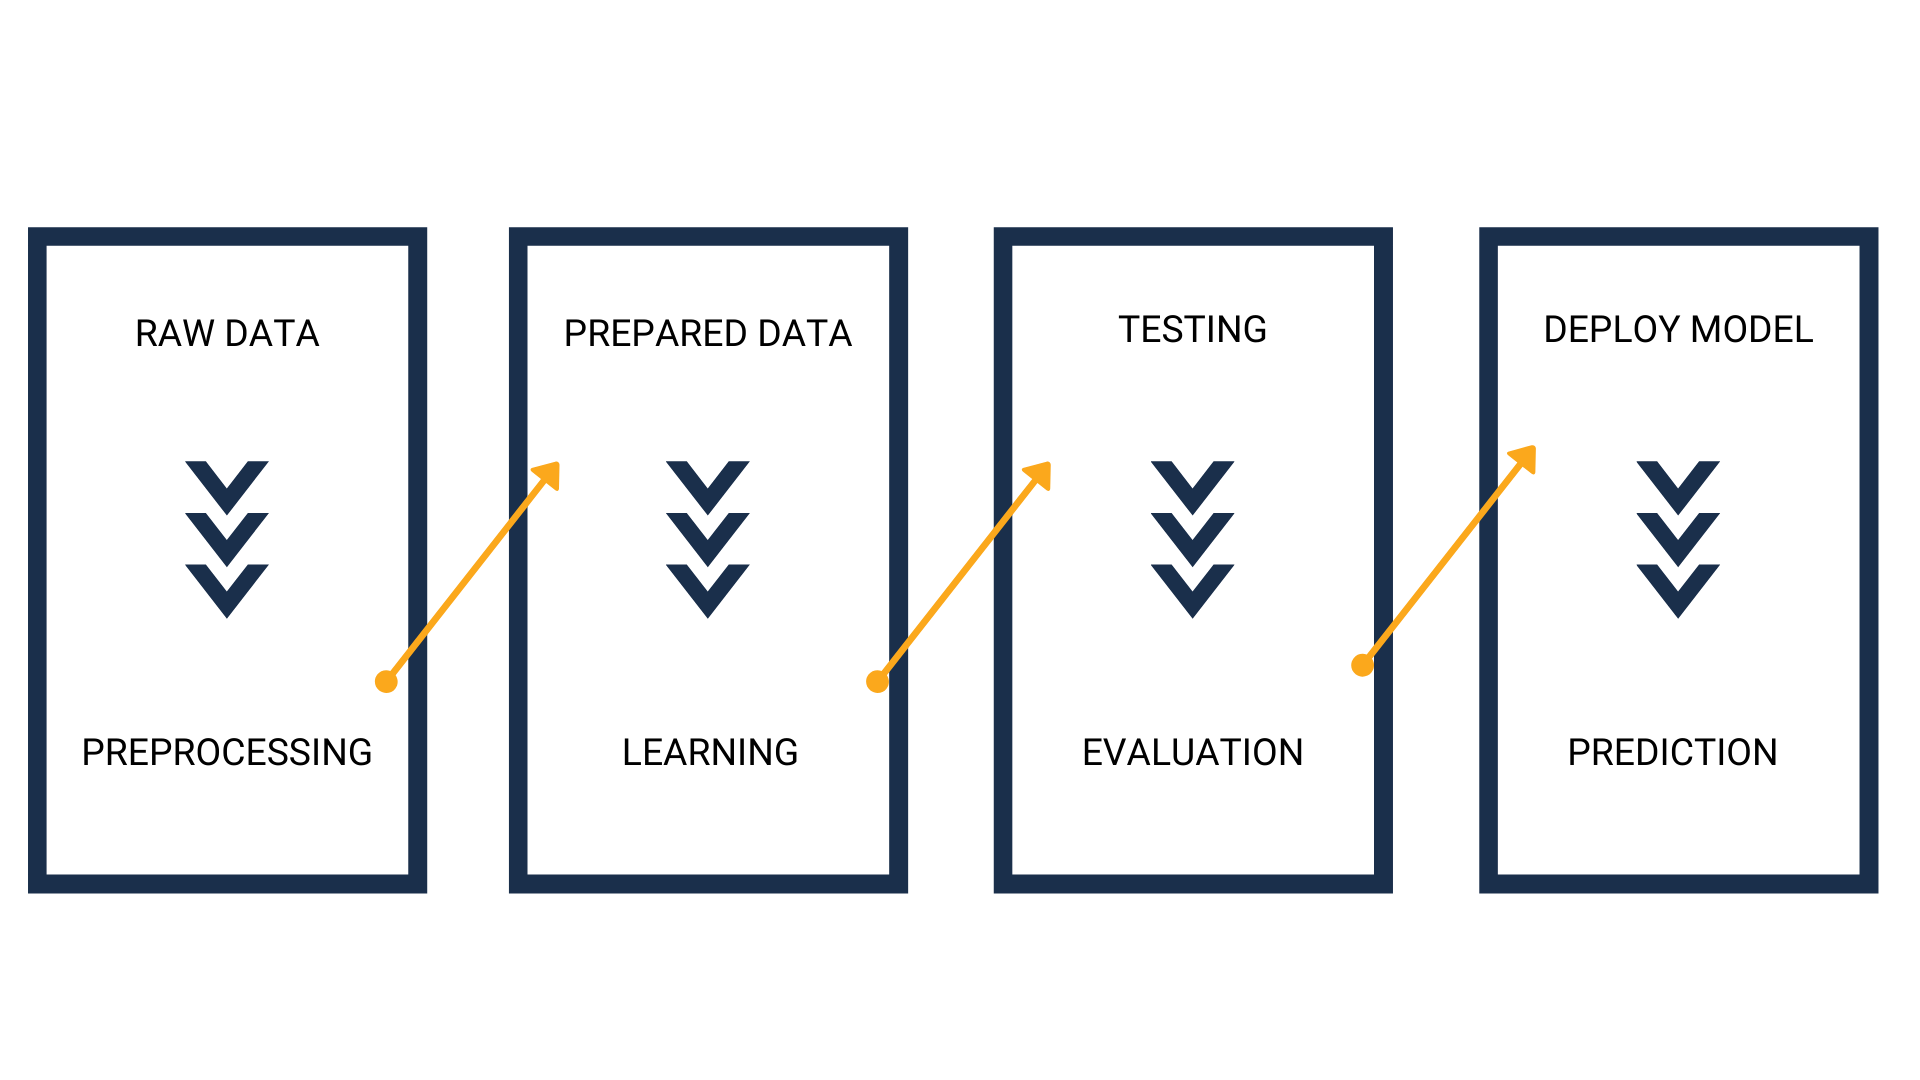
\includegraphics[width=0.7\textwidth]{echosec_machine_learning_diagram.png}
    \caption{A Diagram of a Typical Machine Learning Process. \cite{echosec}}
\end{figure}

\section{Evidence of Machine Learning's Effectiveness}
Machine learning algorithms are already being employed to detect cyberattacks.
The following are a few case studies of machine learning being successfully implemented.

\subsection{Windows Defender Antivirus}
In 2018, a new malware attack campaign was launched against over a thousand users of Windows 7 Pro \cite{microsoft2018}.
The Windows Defender Antivirus features lightweight machine learning models built into the client, which responded immediately to the attack \cite{microsoft2018}.
These models detected a high probability of maliciousness, so they sent data to the Windows Defender Antivirus cloud protection service, which runs more complex machine learning models \cite{microsoft2018}.
Through this, the cloud protection service correctly identified the requests as a cyberattack and responded back to the clients, instructing them to block the attack \cite{microsoft2018}.
The use of machine learning algorithms were able to protect thousands of users from a cyberattack with no human intervention.

\section{Drawbacks of Machine Learning for Cybersecurity}

\section{Discussion}
